Du hast also das Bachelorstudium an der Goethe-Universität begonnen, alle
Achtung für dieses Wagnis! Die ersten Abschlussjahrgänge existieren
mittlerweile, somit bestehen schon einige Erfahrungen innerhalb des
Studiengangs. Sollten dennoch Probleme oder Fragen zu deinem Studium auftreten,
scheue dich nicht, die entsprechenden Verantwortlichen bzw. die Fachschaft
darauf anzusprechen.

Bei einigen formalen Fragen reicht meistens auch schon ein
kurzer Blick in die Bachelorordnung (natürlich in der \textbf{neuen} Version
von 2013)\footnote{\href{http://www.cs.uni-frankfurt.de/images/pdf/informatik/bachelor2/bachelorordnung\_neu.pdf}{http://www.cs.uni-frankfurt.de/images/pdf/informatik/bachelor2/bachelorordnung\_neu.pdf}}.
Damit du beim Studieren der Ordnung nicht völlig verwirrt wirst, haben wir die
wichtigen Informationen zum Bachelorstudium in diesem Artikel kurz zusammengefasst.

Generell wäre es jedoch eine gute Idee, wenn du dir \textbf{die Bachelorordnung zumindest einmal richtig durchlesen} würdest. Damit kann man u.U. einigen (bösen) Überraschungen vorbeugen.

Das Bachelorstudium setzt sich aus einer Reihe von \textbf{Modulen} zusammen, die zu bestehen sind. Ein Modul ist eine inhaltlich und zeitlich abgeschlossene Lehr- und Lerneinheit mit definierten Zielen und Inhalten. Module erstrecken sich in der Regel über ein oder zwei Semester. Falls sich ein Modul über mehr als ein Semester erstreckt, ist es empfehlenswert, die zugehörigen Lehrveranstaltungen in \textbf{unmittelbar aufeinander folgenden Semestern} zu besuchen.

Es kann Zulassungsvoraussetzungen für den Besuch von Veranstaltungen oder die Anmeldungen zur entsprechenden Modulabschlussprüfungen des Moduls geben, die zu beachten sind. Für den Besuch von höheren/späteren Modulen kann z.B. der erfolgreiche Abschluss einiger grundlegender Module ein notwendiges Kriterium sein.

Den Modulen werden Credit Points\footnote{dt. Kreditpunkte, abk. CP} zugeordnet, die dem erwarteten durchschnittlichen Aufwand eines Studierenden für die Veranstaltung (also für den Besuch, die Vor- und Nachbereitung sowie den restlichen Aufwand wie Lösung von Übungsaufgaben oder Teilnahme an einer Übung) wiedergeben sollen. Sie werden auch zur Gewichtung bei der Berechnung der Gesamtnote für den Bachelor verwendet. \textbf{1 CP entspricht dabei in etwa dem Arbeitsaufwand von 30 Stunden}; pro Semester sollen in einem Vollzeitstudium etwa 30 CP erreicht werden (also 900 Stunden Arbeitsaufwand pro Semester).

Allerdings sei hier Vorsicht geboten: Man sollte sich nicht mit Veranstaltungen übernehmen. Es ist schon öfter vorgekommen, dass sich Studierende mit Vorlesungen zugepackt haben und am Ende des Semesters, wegen dem hohen Lernaufwand, größtenteils durchgefallen sind. Beachte: \textbf{Lieber drei Klausuren bestehen, als fünf Klausuren nicht bestehen.} ;)

Bei den Modulen wird zwischen Pflichtmodulen und Wahlpflichtmodulen unterschieden. Während Pflichtmodule (z.B. Basismodule) für den erfolgreichen Abschluss des Bachelors erforderlich sind, kannst du bei den Wahlpflichtmodulen aus einem bestimmten Katalog auswählen. Die Module selbst wiederum bestehen aus Pflicht- und Wahlpflichtveranstaltungen. Auch hier sind die Pflichtveranstaltungen für dich für dieses Modul verbindlich, bei den Wahlpflichtveranstaltungen kannst du eine Auswahl treffen. 

Prüfungen in einem Modul müssen in der Regel \textbf{spätestens 2 Wochen vor dem  Prüfungstermin im Prüfungsamt} angemeldet werden und ein Rücktritt von einer Modulprüfung ist nur bis 1 Woche vor dem Prüfungstermin möglich. Falls ihr mal ein Basismodul in einem Semester nicht bestanden habt, ist es notwendig dieses Modul unbedingt anschließend in einem Zeitraum von 15 Monaten zu wiederholen. Falls ihr das nicht tut, wird es als fehlgeschlagener Wiederholungsversuch gewertet.

Weiter werden die Module verschiedenen Klassen zugeordnet, hierbei gibt es \emph{Basismodule}, \emph{Vertiefungsmodule}, \emph{Anwendungsfachmodule}, \emph{Ergänzungsmodule} und das \emph{Abschlussmodul}. Die Tabellen auf der vorherigen Seite sollen dir eine Übersicht geben, wann der Besuch der entsprechenden Module empfohlen wird.

\begin{center}
	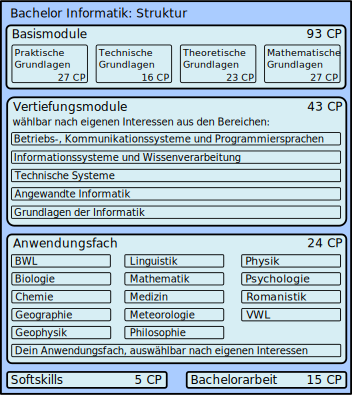
\includegraphics[width=85mm]{bitmaps/bachelor/BacInfStruktur}
\end{center}

Die \textbf{Basismodule} umfassen grundlegende Veranstaltungen der Informatik und der Mathematik. Hierbei werden die Gebiete Programmierung, Hardware, Modellierung, Datenstrukturen, Grundlagen, zwei Praktika in der Informatik und angewandte Mathematik abgedeckt. Bei der angewandten Mathematik musst du drei Veranstaltungen besuchen und abschließen: Mathe-1, Mathe-2 und Mathe-3. Alle Basismodule werden mindestens jährlich angeboten. Wie man in den ersten Semestern vorgehen könnte/sollte, wird aus den Tabellen am Anfang dieses Artikels ersichtlich.

Für die Basismodule gilt die sogenannte \textbf{Freiversuchsregelung}:
\begin{noindEnumerate}
	\item Wenn du eine Modulabschlussprüfung zum ersten mal nicht bestehst, verlierst du keinen Versuch, und die Prüfung gilt für dich als „nicht stattgefunden".
	\item Wenn du sie mit einer Note bestehst, mit der du nicht zufrieden bist, kannst du den \emph{„Freiversuch mit Verbesserungsmöglichkeit''} einsetzen. Dann darfst du die Klausur am nächstmöglichen Termin wiederholen. Angerechnet wird anschließend die beste der beiden Noten. Die Anzahl der Freiversuche mit Verbesserungsmöglichkeit darf im gesamten Studium höchstens fünf betragen.
\end{noindEnumerate}
Dabei ist zu beachten, dass:
\begin{noindEnumerate}
	\item für jedes Basismodul höchstens ein Freiversuch verwendet werden kann
	\item die Freiversuchsregelung nur für die Modulabschlussprüfungen gilt, die innerhalb der  Freiversuchsfrist\footnote{Steht in der Bachelorordnung auf der Beschreibungsseite jedes Basismoduls.\\ Ist außerdem berechenbar: Studienplansemester+1.} gemacht werden.
\end{noindEnumerate}

Die \textbf{Vertiefungsmodule} sind aus folgenden fünf Vertiefungsgebieten auszuwählen:

\begin{noindItemize}
	\item Betriebs- und Kommunikationssysteme und Programmiersprachen und -paradigmen (BKSPP)
	\item Informationssysteme und Wissensverarbeitung (ISWV)
	\item Technische Systeme (TS)
	\item Angewandte Informatik (ANI)
	\item Grundlagen der Informatik (GDI)
\end{noindItemize}
Hier sind mindestens 43 CP zu erbringen.

In einem der Vertiefungsgebiete sind Module im Umfang von mindestens 16 CP, in zwei weiteren Gebieten Module im Umfang von mindestens 8 CP zu erbringen, die verbleibenden CPs können frei aus allen (fünf) Vertiefungsgebieten gewählt werden. Es muss aber insgesamt mindestens ein Seminar und ein Praktikum dabei sein (höchstens drei Seminare und zwei Praktika).

% Das folgende ist veraltet
%Die Wahl dieser drei Vertiefungsgebiete musst du bei der Anmeldung zur ersten Modulabschlussprüfung in einem Vertiefungsgebiet treffen (und dies auch im Prüfungsamt der Informatik angeben). Ein Wechsel ist später möglich, aber in der Regel nur, wenn du noch keine 8~CP in dem Vertiefungsgebiet erreicht hast, welches du abwählst. Sonst ist ein Wechsel nur aus triftigem Grund möglich. Insgesamt dürfen hier Modulabschlussprüfungen, inklusive Wiederholungen, im Umfang von 100 CP abgelegt werden.

Zu beachten ist außerdem, dass Vertiefungsmodule oftmals nur in einem Zweijahresrhythmus angeboten werden, so dass du unter Umständen ein paar Semester warten musst, bis deine „Wunschmodule“ angeboten werden. Ein nützlicher Ratschlag wäre hier den Ablauf deines Studiums einigermaßen zu planen und im Auge zu behalten. Denn wenn du auf einmal am Semesteranfang da stehst und merkst, dass für deine gewählten Vertiefungsgebiete kaum Veranstaltungen angeboten werden, kann das sehr ärgerlich sein. Der Vertiefungsmodulplaner\footnote{\href{http://www.ki.cs.uni-frankfurt.de/BScPlan/v2/}{http://www.ki.cs.uni-frankfurt.de/BScPlan/v2/}} ist dabei sehr nützlich.

Üblicherweise solltest du um das 3-4 Semester noch ein \textbf{Anwendungsfach} belegen (ähnlich einem Nebenfach, das nicht direkt was mit Informatik zu tun hat). Es gibt mittlerweile eine große Auswahl von verschiedenen Anwendungsfächern, einige davon sind z.B. BWL, Biologie, Physik und Philosophie. Die Module in dem von dir gewählten Anwendungsfach sind entsprechend \emph{Anhang II} der Bachelorordnung zu besuchen. Das gewählte Anwendungsfach musst du dem Prüfungsamt mitteilen, erst dann darfst du darin Modulabschlussprüfungen absolvieren. Deshalb kann es nützlich sein, in den ersten Semestern mal in die entsprechenden Veranstaltungen hineinzuschnuppern bzw. ältere Studierende (oder auch die Fachschaftler) über Anwendungsfächer zu fragen. Eine falsche Auswahl ist jedoch hier nicht ganz so dramatisch: wenn du feststellst, dass das Fach nichts für dich ist, ist ein Wechsel des Anwendungsfachs jederzeit möglich.

Im Anwendungsfach sind Veranstaltungen im Wert von 24 CP einzubringen. Die Regelungen zu Modalitäten wie Anmeldefristen oder Wiederholungen hierzu werden vom anbietenden Fachbereich festgesetzt.

Für diejenigen, die etwas ganz Ausgefallenes suchen: Es besteht die Möglichkeit, ein nicht geregeltes Anwendungsfach zu beantragen. Allerdings ist dies ein relativ komplexer Vorgang, der wohl geplant werden muss – also im Zweifel bei jemandem nachfragen, der sich damit auskennt.

Ein \textbf{Ergänzungsmodul} im Umfang von 5 CP muss auch noch absolviert werden. Dieses besteht aus der \textbf{Pflichtveranstaltung (die Studiumsorientierungsveranstaltung ``Einführung in das Studium''), die fürs erste Semester empfohlen wird} und dem Wahlpflichtanteil, wo du eine Auswahl unter der Veranstaltung ``Einführung in das IT-Projektmanagement'', mehreren Soft Skills-Veranstaltungen, der Gremienarbeit, der Tutoriumleitung  und der Leitung eines Mentoriums treffen kannst. Die Wahlpflichtveranstaltungen werden im 5. bzw. 6. Semester empfohlen.

Das \textbf{Abschlussmodul} besteht aus dem Oberseminar und der Bachelorarbeit. Für die Bachelorarbeit hast du 9 Wochen Bearbeitungszeit, sie darf auch nur einmal wiederholt werden. Hier ist es auch möglich, die Arbeit ganz oder teilweise in einer Einrichtung außerhalb der Goethe-Universität anzufertigen. Dieses Modul sollst du laut Studienplan im 6. Semester durchführen, es zählt 15 CP.

Mit diesen insgesamt (mindestens) 180 CP wird dein Studium komplettiert und du erhältst dann deine Urkunde. Die Notenbildung wird hierbei, anhand deiner nach den CP gewichteten Noten in den  Modulabschlussprüfungen gewichtet, geregelt, wobei noch zusätzlich zu einer Vergleichsgruppe relative Noten vergeben werden.

Ganz wichtig zu beachten sind noch weitere Regelungen zum endgültigen Nichtbestehen: \textbf{Bis zum Beginn des vierten Fachsemesters musst du zwei Basismodule  abschließen, sonst bist du leider raus.}

Kommen wir nun zu einigen Formalitäten. Irgendwann im Verlauf des ersten Semesters werdet ihr euch für die ersten Prüfungen anmelden. Damit ihr nicht in Zeitnot bei der Anmeldung geratet, hier ein kleiner Überblick wie ihr euch für welche Prüfungen anmeldet.

\begin{center}
	
\includegraphics[scale=0.8]{bitmaps/bachelor/tests_icon}
\end{center}

% ### Für Wintersemester ###
\textbf{Schriftliche Modulabschlussprüfungen:} Im ersten Semester gibt es die Modulabschlussprüfungen \emph{B-MOD} (Modellierung), \emph{B\hbox{-}PRG1} (Grundlagen der Programmierung 1 und Einführung in die Programmierung) und \emph{B-M1} (Mathematik 1).
% ### Für Sommersemester ###
%\textbf{Schriftliche Modulabschlussprüfungen:} Im ersten Semester gibt es die Modulabschlussprüfungen \emph{B-DS} (Datenstrukturen), \emph{B-PRG2} (Grundlagen der Programmierung 2) und \emph{B\hbox{-}HW1} (Hardwarearchitekturen und Rechensysteme).
Allerspätestens zwei Wochen vor dem Klausurtermin müsst ihr euch im QIS-LSF\footnote{Websystem der Universität für die Verwaltung des Studiums: \href{https://qis.server.uni-frankfurt.de/}{https://qis.server.uni-frankfurt.de/}} dafür anmelden. \textbf{Die Anmeldungsfunktion müsst ihr davor freischalten,} indem ihr ein entsprechendes Formular im Prüfungsamt ausfüllt und abgebt. Vor den Klausuren und Prüfungen herrscht im Prüfungsamt oft ein höherer Betrieb. Man sollte sich deshalb früh genug um die Anmeldung kümmern und nicht erst am letztmöglichen Tag.


\textbf{Anmeldung zu einer mündlichen Modulabschlussprüfung:} Für die mündliche Modulabschlussprüfung müsst ihr zuerst ein entsprechendes Formular im Prüfungsamt besorgen und dann zum Professor gehen, der euch prüfen soll. Dieser Professor wird mit euch einen Prüfungstermin vereinbaren und unterschreibt dann das Formular. In Modulen, in denen die Vorlesung von mehreren Professoren gehalten wurde, könnt ihr euch einen Prüfer aussuchen. Da auch Professoren manchmal Urlaub machen, solltet ihr euch die Prüfungstermine rechtzeitig besorgen.

Abschließend noch 4 Ratschläge, die wir euch für euer Studium dringend mitgeben wollen:

\textbf{1)Lasst euch nicht unterkriegen.}\\
Ein Studium der Informatik ist sicher nicht leicht. Es kommt mit Sicherheit ein großer Lernaufwand auf euch zu, den man nicht unterschätzen sollte. Allerdings sei hier gesagt: Wer das Durchhaltevermögen hat, der kann es auch schaffen.
Also nochmal (auch wenn das heißt sich Zwecks Lernen die Nächte um die Ohren zu schlagen): \textbf{Lasst – euch – nicht – unterkriegen.}

\textbf{2) Besucht regelmäßig eure Vorlesungen und die zugehörigen Tutorien.}\\
Und wenn ihr in einer Vorlesung oder einem Tutorium sitzt, dann passt auch auf. Filme schauen oder Spiele spielen auf dem Laptop ist während einer Veranstaltung die reinste Zeitverschwendung.

\textbf{3) Macht ggf. die Übungsaufgaben!}\\
Damit könnt ihr direkt eure Prüfungsnoten um ein paar Notenstufen verbessern! Außerdem gilt bei uns die Statistik: Wer mindestens 50\% der Übungsaufgaben im Laufe des Semesters gelöst hat, besteht mit 97\% Wahrscheinlichkeit die Klausur.

\textbf{4) Fangt nicht erst 3 Tage vor einer Prüfung an zu lernen.}\\
Ihr studiert an einer Universität und Prüfungen umfassen meistens den Inhalt des ganzen Semesters. Plant euch die Zeit zum Lernen für eure Prüfungen genau ein, denn es ist empfehlenswert oft mind. 2 Wochen vorher anzufangen.\\

\begin{flushright}Claudia, Oliver, Grzegorz, modified by Pavel \end{flushright}
